First of all, some crucial definitions are reported in the following.
\begin{itemize}
    \item \textbf{Computational Neuroscience:} an approach to properly understand the information content of
          neural signals by modelling the nervous system at several different scales. The final goal
          is to bridge the gap between experimental observations of neuronal systems and theoretical
          models.
    \item \textbf{Model:} equations with specified parameters, generally hard to be solved
          analytically.
    \item \textbf{Simulator:} a software which is able to execute or solve a model.
    \item \textbf{Simulation:} the execution of a model into a simulator.
    \item \textbf{Reverse Engineering:} the exploitation of experimental data to build better models
          by inferring some of the parameters.
\end{itemize}
Generalized models are extremely difficult to build and solve, therefore proper simplifying
assumptions are often necessary.\\
Notice that in Computational Neuroscience three different levels of analysis do exist:
\begin{enumerate}
    \item \textit{Computational level}: the problem
    \item \textit{Algorithmic level}: the strategy
    \item \textit{Implementation level}: how it is actually done by networks of neurons
\end{enumerate}
As brain computation is distributed, it is vital to understand how neurons are intertwined and
connected together. A proper simulation should take into account signals at several distinct
scales, not only action potentials, but also LFPs, ECoG, EEG, and so on.
\begin{figure}[H]
    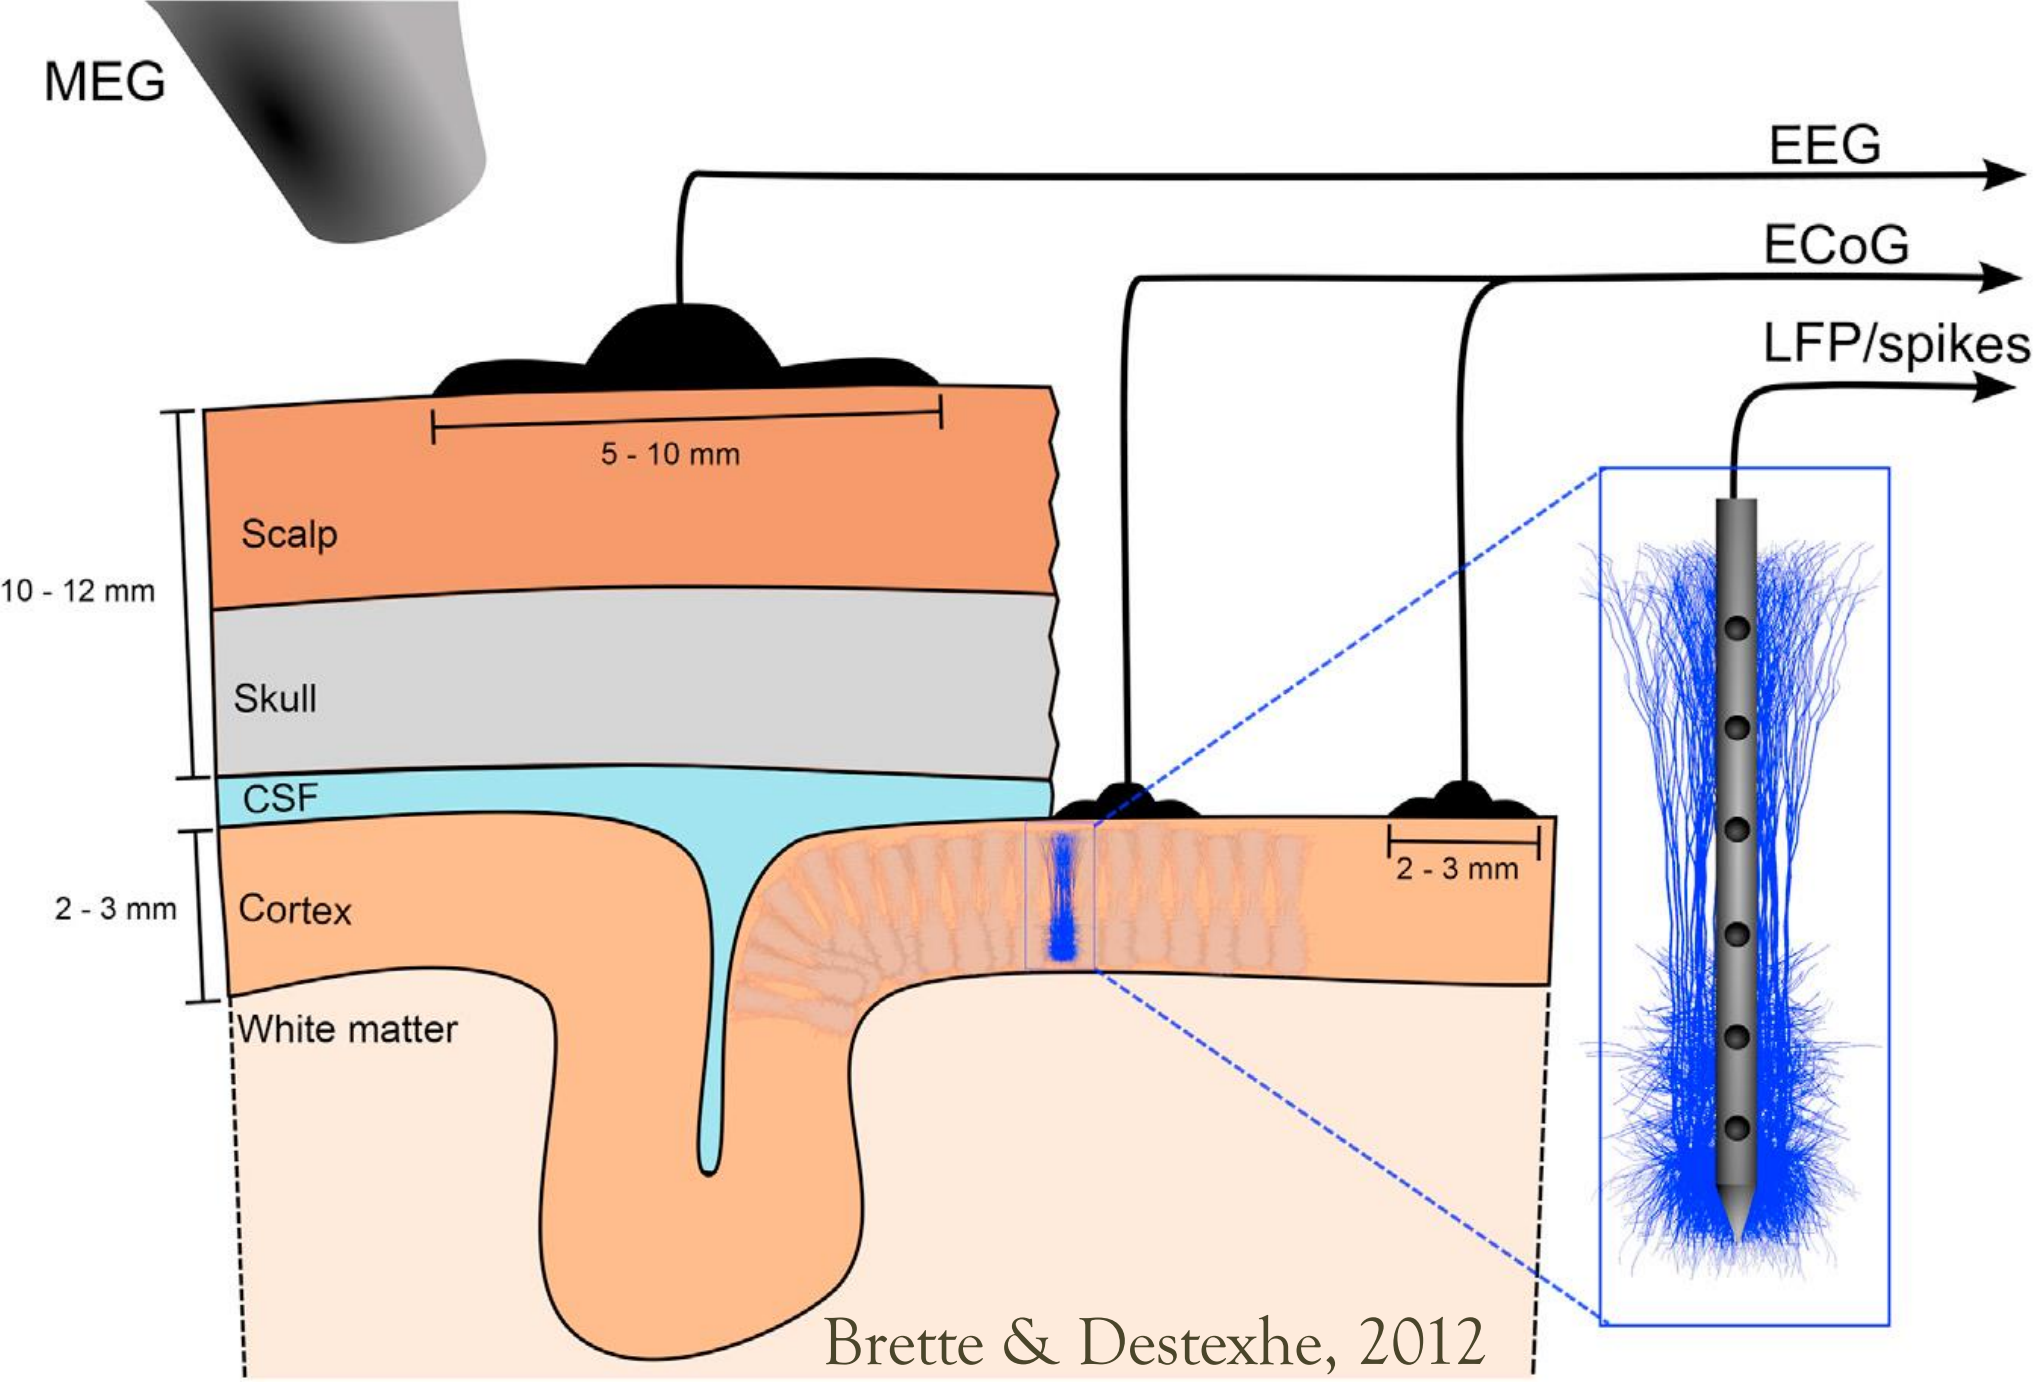
\includegraphics[scale=0.25]{01_1}
    \centering
\end{figure}
Finally, it should be stated that there is still no comprehensive theory describing information
processing in the brain, but important building blocks can be won through these approaches and
may constitute the basis for such a theory in the future.